\documentclass[12pt,fleqn]{article}
\usepackage{xiiiemc}
\usepackage{natbib}
\usepackage{fancyhdr}
\usepackage{fancyvrb}
\usepackage{color}
\usepackage{wallpaper} 
\usepackage{titlesec}   %% Define space between paragraph e section
\usepackage{float} 	%% Use to fix Figure or Table: ex: \begin{table}[H]
\usepackage[usenames,dvipsnames]{xcolor}
\usepackage{hyperref} 	%% Use to fix Figure or Table: ex: \begin{table}[H]
\hypersetup{
	%pagebackref=true,
	pdfcreator={LaTeX with abnTeX2},
	pdfkeywords={abnt}{latex}{abntex}{USPSC}{trabalho acadêmico}, 
	colorlinks=true,       		% false: boxed links; true: colored links
	linkcolor=blue,          	% color of internal links
	citecolor=blue,        		% color of links to bibliography
	filecolor=magenta,      		% color of file links
	urlcolor=blue,
	allbordercolors=black,
	bookmarksdepth=4
}
\usepackage{tocloft}
\titleformat{\section}
  {\normalfont\bfseries}{\thesection.}{0.5em}{}
\renewcommand\cftsecaftersnum{.} 
\renewcommand\thesection{\arabic{section}}
\renewcommand\thesubsection{\thesection.\arabic{subsection}}
%%%%Don't edit this block. It reduces the spacing between the lines of the references
\let\OLDthebibliography\thebibliography
\renewcommand\thebibliography[1]{\OLDthebibliography{#1} \setlength{\parskip}{0pt}\setlength{\itemsep}{0pt plus 0.3ex}}

\usepackage{grffile}
\usepackage{afterpage}

%%-----------------------------------------------EDIT-----------------------------------------------
\title{A distance derived from the Kolmogorov-Smirnov statistic:
	specification, reference measures and example uses}

%%-----------------------------------------------EDIT----------------------------------------------
\author
    {\rm \begin{tabular}{l} 
    \textbf{Renato Fabbri}$$ - {\textnormal renato.fabbri@gmail.com}\\%
    {\fontsize{11}{0}\selectfont University of São Paulo, Institute of Mathematical and Computer Sciences - São Carlos, SP, Brazil}\vspace*{-0.05cm} \\
%    {\fontsize{11}{0}\selectfont $^{2}$Federal University of ABC, Centre for Natural Sciences and Humanities - São Paulo, SP, Brazil}\vspace*{-0.05cm}\\
  \end{tabular}}
%%----------------------------------------------------------------------------------------------

\fancypagestyle{firspagetstyle}
{
	\lhead{}
	\fancyhead[C]{%
		
\includegraphics[width=0.9\linewidth]{logo}\\%
		{\scriptsize \fontfamily{phv}\fontseries{b}\selectfont \color[rgb]{0.45,0.45,0.45}
		16 a 19 de Outubro de 2017\\
		Instituto Politécnico - Universidade do Estado de Rio de Janeiro\\
		Nova Friburgo - RJ\\
	    }
	}
	\renewcommand{\headrulewidth}{0.0pt}
	\fancyfoot[C]{\footnotesize \parbox{15cm} {\centering  \fontsize{7.5}{0}\selectfont \it Anais do XX ENMC – Encontro Nacional de Modelagem Computacional e VIII ECTM – Encontro de Ciências e Tecnologia de Materiais,  Nova Friburgo, RJ – 16 a 19 Outubro 2017}} % \ttfamil
	\rhead{}
}


\begin{document}
\maketitle

\thispagestyle{firspagetstyle}

\fancyhead[L]{\footnotesize{\fontsize{7.5}{0}\selectfont \it XX ENMC e VIII ECTM\\
	16 a 19 de Outubro de 2017\\
	Instituto Politécnico Universidade do Estado do Rio de Janeiro – Nova Friburgo - RJ\\}}
\renewcommand{\headrulewidth}{0.0pt}
\fancyfoot[C]{\footnotesize \parbox{15cm} {\centering  \fontsize{7.5}{0}\selectfont \it Anais do XX ENMC – Encontro Nacional de Modelagem Computacional e VIII ECTM – Encontro de Ciências e Tecnologia de Materiais,  Nova Friburgo, RJ – 16 a 19 Outubro 2017}} % \ttfamil
\rhead{}

\begin{abstract}
Statistical distances quantifies the difference between two statistical constructs.
In this article, we describe reference values for a semimetric
derived from the Kolmogorov-Smirnov statistic $D_{F,F'}$.
Each measure of the $D_{F,F'}$ is a distance between two histograms.
This distance is normalized by the number of observations in each sample
to yield the $c'=D_{F,F'}\sqrt{\frac{n n'}{n+n'}}$ statistic,
which can be mapped to p-values, i.e. values for which 
high enough levels of significance $\alpha$ implies the rejection of the
	null hypothesis (that the samples are drawn from the same distribution).
One great feature of $c'$ is that it inherits the robustness of
	$D_{F,F'}$ and is thus suitable for use in settings where
	the underlying distributions are not known.
Benchmarks are derived by comparing samples from standard distributions.
The supplied example applications of the $c'$ statistic for the distinction
	of samples in real data enables further
insights about the robustness and power of $c$.
\end{abstract}

\keywords{\em{Statistical distance, Statistics, Kolmogorov-Smirnov test, Statistical test, Benchmark}}

\pagestyle{fancy}

\section{INTRODUCTION}\label{sec:intro}
To quantify the difference between samples that are regarded as statistical events,
one can rely in statistical distances.
Such distances are often not metrics, cases in which they fail in one of
the properties of a metric $m$ on sets $x_i \in X$:
\begin{align}
	m(x_i,x_j) &  \geq 0 \\
	m(x_i,x_j) &  = 0 \Leftrightarrow x_i = x_j \\
	m(x_i,x_j) &  = m(x_j,x_i)\\
	m(x_i,x_j) &  \leq m(x_i,x_z) + m(x_z,x_j)
\end{align}

Pseudometrics violate property (1) and/or (2),
quasimetrics violate property (3),
semimetrics violate property (4).
A divergence only satisfies properties (1) and (2).
These are ``generalized metrics''.

In this article, a statistical distance derived from the
Kolmogorov-Smirnov statistic is described.
To enable the use of the (generalized) metric,
benchmarks are provided
by using standard distributions in various settings and sample sizes.
Example applications of the metric to quantify the difference among
real signals further validate the approach.

Section~\ref{sec:met} describe the metric
and the methods used to characterize it.
Section~\ref{sec:res} is dedicated to
summarizing the results and essential discussions.
Final remarks, including potential future works,
are stated in Section~\ref{sec:res}.


\section{METHODS}\label{sec:met}
This section describes the $c'$ statistical distance,
the strategy of benchmarking and to validate $c'$ by means
of application to real samples.


\subsection{Description of the $c'$ statistic}
Be $F$ and $F'$ two empirical cumulative distributions,
where $n$ and $n'$ are the number of observations in each sample.
The two-sample Kolmogorov-Smirnov test rejects the null hypothesis,
that the histograms are the outcome of the same underlying distribution,
if:
\begin{equation}\label{eq:ks}
D_{F,F'} > c(\alpha)\sqrt{\frac{n+n'}{nn'}}
\end{equation}

\noindent where $D_{F,F'}=sup_x[F-F']$ as in Figure~\ref{fig:dnn}
and $c(\alpha)$ is related to the level of significance $\alpha$ by:

\begin{table}[h!]
\centering
\begin{tabular}{|l||c|c|c|c|c|c|}\hline
$\alpha$    & 0.1  & 0.05 & 0.025 & 0.01 & 0.005 & 0.001 \\\hline
$c(\alpha)$ & 1.22 & 1.36 & 1.48  & 1.63 & 1.73  & 1.95  \\\hline
\end{tabular}
\end{table}

If distributions are drawn from empirical data, $D_{F,F'}$ is given as are $n$ and $n'$.
All terms in equation~\ref{eq:ks} are positive and $c(\alpha)$ can be isolated:

\begin{equation}\label{eq:ks2}
%	c(\alpha) < \frac{D_{F,F'}}{\sqrt{\frac{n+n'}{nn'}}} = c
	c(\alpha) < D_{F,F'}\sqrt{\frac{nn'}{n+n'}} = c'
\end{equation}

%Tables~\ref{tab:kolSub}-\ref{tab:kolPctInter} are populated with values for $c'(\alpha)$
The higher $c'$ is, the lower $\alpha$ can be and still entail the rejection of the null hypothesis.

\begin{figure}[!h]
	\centering
	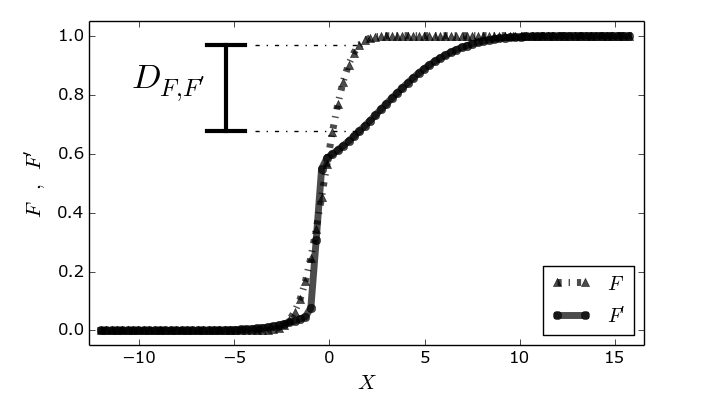
\includegraphics[width=0.44\textwidth]{../figs/Dnn}
	\caption{The Kolmogorov-Smirnov statistic $D_{F,F'}$: the maximum difference between
		two cumulative distribution functions.}
	\label{fig:dnn}
\end{figure}

In summary,
high values of $c$ favor rejecting the null hypothesis.
For example, if the significance level is $\alpha=0.01$,
then $c'$ greater than $1.7$
implies the rejection of the null hypothesis,
i.e. assuming that $F$ and $F'$
are outcomes of different distributions.

Of core importance in this study is to regard $c'$
as a measure of distance between both distributions~\cite{kolm}.
If fact, it is a statistical distance.
Following the concepts defined in Section~\ref{sec:intro},
it is a generalized metric.
It obviously satifies the Equations (1) and (3).
It satisfies Equation (4) for less obvious reasons.
To grasp how $c'$ satisfies Equation (4),
let $x_i$, $x_j$ and $x_z$ be samples of the same size,
so we only need to compare the $D_{F,F'}$.
Let $F_i$ be the cumulative distribution of the sample $x_i$.
Supose that in the value $\xi$ of X where $F_i$ and $F_j$ are maximally different (i.e. where they yield $D_{F_i,F_j}$),
they are also maximaly different against $F_z$.
If the value of $F_z(\xi)$ is between $F_x(\xi)$ and $F_j(\xi)$:
$D_{F_i,F_z}+D_{F_j,F_z} = D_{F_i,F_j}$,
otherwise:
$D_{F_i,F_z}+D_{F_j,F_z} > D_{F_i,F_j}$.
If the KS statistic $D_{F,F'}$ are not yield at the same sample value,
it is because they are larger than in the previous cases, thus:
$D_{F_i,F_z}+D_{F_j,F_z} > D_{F_i,F_j}$.
And this completes the argument for:
$D_{F_i,F_z}+D_{F_j,F_z} \geq D_{F_i,F_j}$.
The $c'$ statistic might satisfy or violate Equation (2),
depending on how it is achieved.
If the obtainance of $c'$ depends on making histograms,
than a slightly different observation of a sample might fall under the same bin.
In this case, $c'=m(x_i,x_j) = 0$ and $x_i \neq x_j$, which violates (2)\footnote{If
we instead regard $x_i$ as a histogram, not a sample,
that it satifies (2), but we here assume that $c'$
is in fact a measure related to samples.}.
The cumulative distributions might be derived, however,
not by making a histogram, but by ordering the samples directly~\citep{stack}.
In this case, $c'$ satifies (2).
One exception: if $x_j$ has twice but the same observations as $x_i$,
then it violates (2).
In other words, the distributions entailed by the samples are the same,
but the samples are not the same, and the distance is still zero.

In summary, if we regard $c'$ as a distance between histograms or distributions,
than it is a metric satisfying all Equations (1-4).
Otherwise it is a pseudometric because it violates Equation (2).

\subsection{Benchmarks obtainance}
We considered two cases: when the null hypothesis (that the samples were drawn from the same underlying distributions)
is true and when it is false.
In the case where the null hypothesis was true, 
we compared similar distributions in various settings
many times to assert that we would not assume
that the null hypothesis was false more than
$\alpha . N_c$ where $\alpha$ is the significance level
and $N_c$ is the number of comparisons.
That is, to assert that the Kolmogorov-Smirnov test results
are in accordance with the theory.

In the case where the null hypothesis was false, 
we were interested in measures of $c'$ given that
the null hypothesis is never rejected for a small enough
$\alpha$.
The various measures performed for $c'$ are
described in the results.

One important aspect of the way by which we made the
benchmarks available is that the rendering of the tables
is automated by configurable scripts,
allowing one to obtain tables with other measures
and other comparisons.

\section{RESULTS AND DISCUSSION}\label{sec:res}
This section briefly describes each of the
results, which are: benchmark tables, example uses of the test in
real samples, an exposition of all the data obtained,
and configurable scripts for the generation of all reference tables.

\subsection{When the null hypothesis is true}
The theory of the Kolmogorov-Smirnov test
states that one can choose a significance value $\alpha$,
which is the maximum probability that one will reject the
null hypothesis while it is true.
Accordingly,
We rendered a table for each of the distributions:
normal, uniform, 1-parameter Weibull, power.
Three to five different settings of the distributions
were used, both samples had a size of 1000 observations,
and $N_c=100$ comparisons were performed.

Table~\ref{tab:true} is one of such tables.
To understand the columns, notice that
if the null hypothesis is true, the number
of rejections of the null hypothesis ($c'>c(\alpha)$)
in $N_c$ comparisons should not exceed $\alpha . N_c$.
To verify this, let $C=\{c'_i\}$ be a set of $c'$ measures,
and $C(\alpha)=\{c' : c'>c(\alpha)\}$.
Be $|C(\alpha)|$ the cardinality of $C(\alpha)$,
i.e. the number of comparisons in which the two-sample Kolmogorov-Smirnov
test rejects the null hypothesis for a given $\alpha$.

The overall result is that, in fact, the false rejections of the null hypothesis
does not exceed $\alpha . N_c$.
The only exception in our simulations is the power-law distribution,
in which the number of rejections of the null hypothesis were usually bellow $\alpha . N_c$
but, in extreme cases, our simulations reached almost $2\alpha N_c$.

\begin{table}[h!]
\begin{center}
\begin{tabular}{| l | c | c | c | c | c | c |}\hline
$\alpha N_c$ & $\alpha$ & $c(\alpha)$ & $|C_1(\alpha)|$ & $|C_2(\alpha)|$ & $|C_3(\alpha)|$ & $|C_4(\alpha)|$ \\\hline\hline
10.0 & 0.100 & 1.22 & 0 & 4 & 3 & 8 \\\hline
5.0 & 0.050 & 1.36 & 0 & 0 & 1 & 3 \\\hline
2.5 & 0.025 & 1.48 & 0 & 0 & 0 & 0 \\\hline
1.0 & 0.010 & 1.63 & 0 & 0 & 0 & 0 \\\hline
0.5 & 0.005 & 1.73 & 0 & 0 & 0 & 0 \\\hline
0.1 & 0.001 & 1.95 & 0 & 0 & 0 & 0 \\\hline
\end{tabular}
\caption{The theoretical maximum number $\alpha N_c$ of rejections
of the null hypothesis for critical values of $\alpha$.
The $c_1$ values were calculated using simulations of 1-parameter Weibull distributions with $a=0.1$.
The $c_2$ values were calculated using simulations of 1-parameter Weibull distributions with $a=2$.
The $c_3$ values were calculated using simulations of 1-parameter Weibull distributions with $a=4$.
Over all $N_c$ comparisons,
The $N_o$ values of $c_4$ were calculated using simulations of
 1-parameter Weibull distributions with $a=6$.
Over all $N_c$ comparisons,
 $\mu(c_1)=0.0655$ and $\sigma(c_1)=0.0376$,
 $\mu(c_2)=0.7053$ and $\sigma(c_2)=0.2261$,
 $\mu(c_3)=0.6905$ and $\sigma(c_3)=0.2460$ .
 $\mu(c_4)=0.7596$ and $\sigma(c_4)=0.2644$ .
}
\end{center}
\end{table}

\subsection{When the null hypothesis is false}\label{sec:false}
In this case we are interested in measures of $c'$.
The number of comparisons is still $N_c=100$.
The measures on $c'$ chosen to report the results are:
the mean $\mu(c')$, the standard deviation $\sigma(c')$,
the median $m(c')$,
the  fraction
$\overline{C(\alpha)}=\frac{|C(\alpha)|}{N_c}$
of rejection of the null hypothesis given the significance level $\alpha$.
$min(c')$ states the three smallest values found in the simulations while
$max(c')$ states the three greatest values.
The null hypothesis is true in the boldface lines.
$D$ is the KS statistic when sample size goes to infinity.

Two sets of tables were made to study the $c'$ statistic when
the null hypothesis is false:
\begin{itemize}
	\item Changing the distrubutions: inn each table, the comparisons were made with
one of the distributions remaining unchanged
while the other changes in each row.
Table~\ref{tab:false1} is an example of such table.
	\item Changing the sample sizes:
		changing the number of elements in each sample
		changes the value of the $c$ statistic. 
		The $c$ statistic is given for two samples of varied sizes but
		with fixed underlying distributions.         
		Table~\ref{tab:false2} is an example of such table.
\end{itemize}

\begin{table*}[h!]
\caption{Measurements of $c'$ through simulations
        with power function distributions.
        One power distribution has the fixed exponent parameter $a-1=0.5$.
        The other power function distribution
	has a different value of $a$ in each row (i.e. in each set of $N_c$ comparisons).
	A description of the measures is in Section~\ref{sec:false}.
	}\label{tab:false1}
\tiny
\begin{center}
\begin{tabular}{ l | c | c | c | c | c | c | c | c | c | c | c }
$a$ & $\mu(c')$ & $\sigma(c')$ & min(c') & max(c') & $D$ & $\mu(D_{F,F'})$ & $\sigma(D_{F,F'})$ & $\overline{C(0.1)}$ & $\overline{C(0.05)}$ & $\overline{C(0.01)}$ &  $\overline{C(0.001)}$ \\\hline
0.7 & 6.282 & 0.402 & 4.919,5.299,5.501 & 6.909,6.999,7.021  & 0.274  & 0.281  & 0.018  & 1.000  & 1.000 & 1.000  & 1.000 \\
0.9 & 4.445 & 0.452 & 3.511,3.600,3.622 & 5.344,5.367,5.590  & 0.186  & 0.199  & 0.020  & 1.000  & 1.000 & 1.000  & 1.000 \\\hline
1.1 & 2.818 & 0.443 & 1.588,1.744,1.945 & 3.734,3.846,4.137  & 0.114  & 0.126  & 0.020  & 1.000  & 1.000 & 0.990  & 0.970 \\
1.3 & 1.536 & 0.407 & 0.783,0.827,0.894 & 2.415,2.437,2.549  & 0.053  & 0.069  & 0.018  & 0.750  & 0.650 & 0.350  & 0.170 \\\hline
{\bf 1.5} & {\bf 0.776} & {\bf 0.237} & {\bf 0.425,0.447,0.470} & {\bf 1.409,1.409,1.565} & {\bf 0.000} & {\bf 0.035} & {\bf 0.011} & {\bf 0.060} & {\bf 0.040} & {\bf 0.000} & {\bf 0.000} \\\hline
1.7 & 1.499 & 0.377 & 0.648,0.738,0.850 & 2.281,2.326,2.370  & 0.046  & 0.067  & 0.017  & 0.740  & 0.660 & 0.380 & 0.110 \\\
1.9 & 2.246 & 0.400 & 0.939,1.386,1.521 & 2.952,3.063,3.309  & 0.087  & 0.100  & 0.018  & 0.990  & 0.990 & 0.940 & 0.780 \\\hline
2.1 & 3.051 & 0.395 & 2.393,2.393,2.415 & 3.846,3.891,3.913  & 0.123  & 0.136  & 0.018  & 1.000  & 1.000 & 1.000 & 1.000 \\\
2.3 & 3.710 & 0.442 & 2.683,2.795,2.907 & 4.696,4.718,4.785  & 0.156  & 0.166  & 0.020  & 1.000  & 1.000 & 1.000 & 1.000 \\\hline
2.5 & 4.415 & 0.422 & 3.019,3.175,3.287 & 5.121,5.188,5.210  & 0.186  & 0.197  & 0.019  & 1.000  & 1.000 & 1.000 & 1.000 \\
\end{tabular}
\end{center}
\end{table*}


\begin{table*}[h!]
\caption{Measurements of $c$ through simulations
        with fixed normal distributions but different number of samples.
        One normal distribution has $\mu=0$ and $\sigma=1$.
        The other normal distribution has
        $\mu=0$ and $\sigma=1.2$.
        The KS statistic of these distributions converges
        to 0.0440 as sample sizes increases.
	A description of the measures is in Section~\ref{sec:false}.
	}\label{tab:false2}
\tiny
\begin{center}
\begin{tabular}{ l | c | c | c | c | c | c | c | c | c | c }
$n=n'$ & $\mu(c')$ & $\sigma(c')$ & $m(c')$ & $min(c')$ & $max(c')$ & $\mu(D_{F,F'})$ & $\sigma(D_{F,F'})$ & $\overline{C(0.1)}$ & $\overline{C(0.01)}$ & $\overline{C(0.001)}$ \\\hline
{\bf 100} & 0.911 & 0.251 & 0.849 & 0.424,0.495,0.495 & 1.414,1.626,1.697 & 0.129 & 0.035 & 0.130 & 0.010 & 0.000 \\
{\bf 1000} & 1.466 & 0.260 & 1.431 & 0.917,1.051,1.051 & 1.990,2.080,2.214 & 0.066 & 0.012 & 0.820 & 0.270 & 0.050 \\\hline
{\bf 10000} & 3.467 & 0.243 & 3.465 & 2.878,2.970,2.991 & 3.946,4.080,4.094 & 0.049 & 0.003 & 1.000 & 1.000 & 1.000 \\
{\bf 100000} & 10.129 & 0.253 & 10.125 & 9.595,9.595,9.631 & 10.713,10.735,10.896 & 0.045 & 0.001 & 1.000 & 1.000 & 1.000 \\
\end{tabular}
\end{center}
\end{table*}





\subsubsection{Varying the sample sizes}
\subsection{Example application to real samples}
\subsection{A thorough exposition of the tables}
\subsection{Scripts for automated generation of the tables}

\section{CONCLUSIONS AND FURTHER WORK}\label{sec:conc}
% discrete vs continous

% are histograms really needed?

% make a better presentation of the benchmark tables

% organize the scripts



\subsection*{\textit{Acknowledgements}}
The authors thank CNPq and FAPESP for the funding received while researching the topic of this article,
the researchers of IFSC/USP and ICMC/USP for the recurrent collaboration in every situation
where we needed directions for investigation.

% ------------------------------------------------------------------------
\begin{thebibliography}{99}
\fontsize{11}{0}\selectfont
\bibitem[DrV, 2016]{stack}
	DrV (2016). Python script to obtain the CDF from samples without doing the histogram.
		Stack Overflow.
		From \url{https://stackoverflow.com/questions/24788200/calculate-the-cumulative-distribution-function-cdf-in-python}

\bibitem[Fabbri, 2017]{enhance}
	Fabbri, R. (2017). Enhancements of linked data expressiveness for ontologies.
		Encontro Nacional de Modelagem Computacional 2017 (XX ENMC).
		From \url{https://github.com/ttm/ontologyEnhancements/raw/master/article.pdf}

\bibitem[Heath \& Bizer, 2011]{ldb}
	Heath, T. \& Bizer, C. (2011). Linked Data: Evolving the Web into a Global Data Space (1st edition). Synthesis Lectures on the Semantic Web: Theory and Technology, 1:1, 1-136. Morgan \& Claypool.

\bibitem[Lehmann et al., 2015]{dbpedia}
	Lehmann, J., Isele, R., Jakob, M., Jentzsch, A., Kontokostas, D., Mendes, P. N., ... \& Bizer, C. (2015). DBpedia–a large-scale, multilingual knowledge base extracted from Wikipedia. Semantic Web, 6(2), 167-195.

\bibitem[Munzner, 2014]{munzner}
	Munzner, T. (2014). Visualization analysis and design. CRC press.

\bibitem[W3C, 2010]{w3cld}
	W3C (2017). LINKED DATA CURRENT STATUS, from \url{https://www.w3.org/standards/techs/linkeddata}

\bibitem[Ward et al., 2010]{ward}
	Ward, M. O., Grinstein, G., \& Keim, D. (2010). Interactive data visualization: foundations, techniques, and applications. CRC Press.

\bibitem[Wikipedia, 2017]{wikipData}
	Data. (2017, August 21). In Wikipedia, The Free Encyclopedia. Retrieved
		22:31, August 21, 2017
		, from \url{https://en.wikipedia.org/w/index.php?title=Data&oldid=796493851}

\end{thebibliography}
% ------------------------------------------------------------------------

%For papers written in Portuguese or Spanish.

%\begin{center}
%  TITLE IN ENGLISH
%\end{center}

%\def\abstractname{Abstract}%

%\begin{abstract}
%   Abstract in english
%\end{abstract}

%\keywords{\em{Keywords in english}}

\end{document}
